\documentclass[10pt,a4paper]{article}

\usepackage{amssymb}
\usepackage[french,english]{babel}
\usepackage[utf8]{inputenc}
\usepackage{graphicx}
\usepackage{lineno}
\usepackage{cite}
\usepackage{float}
\usepackage{ccaption}
\usepackage{caption}
\usepackage{array}
\usepackage{lscape}
\usepackage[hmargin=2cm,vmargin=2cm]{geometry}
\usepackage{fancyvrb}
\usepackage{hyperref}

\title{\bf \Large A short manual for {\tt sNMF}:
a program to estimate ancestry coefficients\\
\large (command-line version)
}

\author{
        Eric Frichot (eric.frichot@imag.fr)\\
        Olivier François (olivier.francois@imag.fr)\\
}

\newcommand{\bp}{\mathbf{p}}
\newcommand{\LLL}{\mathcal{L}}

%% BEGIN DOC
\begin{document}


\maketitle
\begin{center}
{\it Please, print this reference manual only if it is necessary.}
\end{center}

\noindent
This short manual aims to help users to run {\tt sNMF} command-line engine on Mac and Linux. 

\section{Description} 
Inference of individual ancestry coefficients, which is important for population genetic and association studies, is commonly performed using computer-intensive likelihood algorithms. With the availability of large population genomic data sets, fast versions of likelihood algorithms have attracted considerable attention. 
\noindent
{\tt sNMF} is a fast and efficient method for estimating individual ancestry coefficients based on sparse non-negative matrix factorization algorithms. In [1], the performances of {\tt sNMF} were compared to the likelihood algorithm implemented in the computer program {\tt ADMIXTURE}.  Without loss of accuracy, {\tt sNMF} computed estimates of ancestry coefficients with run-times approximately 10 to 30 times shorter than those of {\tt ADMIXTURE}.
\\
\\
\noindent
[1] Eric Frichot, François Mathieu, Théo Trouillon, Guillaume Bouchard, Olivier François. (2014) {\it Fast and efficient estimation of individual ancestry coefficients}. Genetics 196: 973 -- 983. 

\section{Installation} 

\noindent
To install the {\tt sNMF} command-line version, unzip the sNMF\_CL.zip file, and run the 
install script (install.command) from the {\tt sNMF} directory.
From a terminal shell, go to the {\tt sNMF} main directory and type ``./install.command''.
If the script is not executable, type ``chmod +x install.command'' and then ``./install.command''.
A set of binaries should be created in the {\tt bin} directory.

\section{Data format}

\subsection{input file}
The {\tt sNMF} input file consists of a single genotype file in the {\bf geno} format. 
\begin{itemize}
\item {\bf geno} (example.geno)

The {\bf geno} format has one row for each SNP.
  Each row contains 1 character per individual:
  0 means zero copies of the reference allele.
  1 means one copy of the reference allele.
  2 means two copies of the reference allele.
  9 means missing data.

Below, an example of a geno file for $n=3$ individuals and $L=4$ loci.
\begin{center}
\footnotesize
\begin{Verbatim}[frame=single]
112
010
091
121
\end{Verbatim}
\end{center}
\end{itemize}

\noindent
{\tt sNMF} also proposes C functions to convert the following formats to the geno format.
\begin{itemize}
\item {\bf ped} (example.ped)

The {\bf ped} format has one row for each individual. Each row contains 6 columns of information for each individual, plus two genotype columns for each SNP. Each column must be separated by spaces or tabulations. Genotype format must be either 0ACGT or 01234, where 0 means missing data. The first 6 columns of the genotype file are: 1st column is family ID, 2nd column is sample ID, 3rd and 4th columns are sample IDs of parents, 5th column is gender (male is 1, female is 2), 6th column is case/control status (1 is control, 2 is case), quantitative trait value or population group label. 
The ped format is also described at the following \href{http://pngu.mgh.harvard.edu/~purcell/plink/data.shtml#ped}{link}.

Below, an example of a ped file for $n=3$ individuals and $L=4$ loci.
\begin{center}
\footnotesize
\begin{Verbatim}[frame=single]
1 SAMPLE0 0 0 2 2 1 2 3 3 1 1 2 1
2 SAMPLE1 0 0 1 2 2 1 1 3 0 4 1 1
3 SAMPLE2 0 0 2 1 2 2 3 3 1 4 1 2
\end{Verbatim}
\end{center}

The format of the command line is:
\begin{Verbatim}[frame=single]
./bin/ped2geno  input_file [output_file]
\end{Verbatim}
where 
\begin{itemize}
\item \verb|input_file| is the path for the input file (in ped format).
\item \verb|output_file| is the path for the output\_file (in geno format). 
By default, the name of the output file is the name of the input\_file with the .geno extension.

\end{itemize}

\item {\bf ancestrymap} (example.ancestrymap)\\
The {\bf ancestrymap} format has one row for each genotype. Each row has 3 columns: 1st column is SNP name, 2nd column is sample ID, 3rd column is number of alleles. It is assumed that the genotypes for a given SNP name are written in consecutive lines. It is also assumed that the genotypes for a set of individuals are given in the same order as lines. The number of alleles can be the number of reference alleles or the number of derived alleles as long as it is the same choice for an entire SNP. It is assumed that missing genotypes are encoded by the value 9.

Below, an example of an ancestrymap file for $n=3$ individuals and $L=4$ loci.
\begin{center}
\footnotesize
\begin{Verbatim}[frame=single]
rs0000  SAMPLE0 1
rs0000  SAMPLE1 1
rs0000  SAMPLE2 2
rs1111  SAMPLE0 0
rs1111  SAMPLE1 1
rs1111  SAMPLE2 0
rs2222  SAMPLE0 0
rs2222  SAMPLE1 9
rs2222  SAMPLE2 1
rs3333  SAMPLE0 1
rs3333  SAMPLE1 2
rs3333  SAMPLE3 1
\end{Verbatim}
\end{center}

The format of the command line is:
\begin{Verbatim}[frame=single]
./bin/ancestrymap2geno  input_file [output_file]
\end{Verbatim}
where 
\begin{itemize}
\item \verb|input_file| is the path for the input file (in ancestrymap format).
\item \verb|output_file| is the path for the output\_file (in geno format). 
By default, the name of the output file is the name of the input\_file with the .geno extension.
\end{itemize}

\item {\bf vcf} (example.vcf)\\
The {\bf vcf} format is described at the following \href{http://www.1000genomes.org/wiki/Analysis/Variant\%20Call\%20Format/vcf-variant-call-format-version-41}{link}.

Below, an example of vcf file for $n=3$ individuals and $L=4$ loci.
\begin{center}
\footnotesize
\begin{Verbatim}[frame=single]
##fileformat=VCFv4.1 
##FORMAT=<ID=GM,Number=1,Type=Integer,Description="Genotype meta"> 
##INFO=<ID=VM,Number=1,Type=Integer,Description="Variant meta"> 
##INFO=<ID=SM,Number=1,Type=Integer,Description="SampleVariant meta"> 
#CHROM POS ID REF ALT QUAL FILTER INFO FORMAT SAMPLE0 SAMPLE1 SAMPLE2 
1 1001 rs0000 T C 999 . VM=1;SM=100 GT:GM 1/0:1 0/1:2 1/1:3 
1 1002 rs1111 G A 999 . VM=2;SM=101 GT:GM 0/0:6 0/1:7 0/0:8 
1 1003 notres G AA 999 . VM=3;SM=102 GT:GM 0/0:11 ./.:12 0/1:13 
1 1004 rs2222 G A 999 . VM=3;SM=102 GT:GM 0/0:11 . 1/0:13
1 1003 notres GA A 999 . VM=3;SM=102 GT:GM 0/0:11 ./.:12 0/1:13 
1 1005 rs3333 G A 999 . VM=3;SM=102 GT:GM 1/0:11 1/1:12 0/1:13 
\end{Verbatim}
\end{center}

The format of the command line is:
\begin{Verbatim}[frame=single]
./bin/vcf2geno  input_file [output_file]
\end{Verbatim}
where 
\begin{itemize}
\item \verb|input_file| is the path for the input file (in vcf format).
\item \verb|output_file| is the path for the output\_file (in geno format). 
By default, the name of the output file is the name of the input\_file with the extension .geno.
\end{itemize}

\item {\bf lfmm} (example.lfmm)\\
The {\bf lfmm} format has one row for each individual. Each row contains one value for each locus (separated by spaces or tabulations): the number of alleles. The number of alleles can be the number of reference alleles or the number of derived alleles. Missing genotypes are encoded by the values 9 or -9. 


Below, an example of a lfmm file for $n=3$ individuals and $L=4$ loci.
\begin{center}
\footnotesize
\begin{Verbatim}[frame=single]
1 0 0 1
1 1 -9 2
2 0 1 1
\end{Verbatim}
\end{center}

The format of the command line is:
\begin{Verbatim}[frame=single]
./bin/lfmm2geno  input_file [output_file]
\end{Verbatim}
where 
\begin{itemize}
\item \verb|input_file| is the path for the input file (in lfmm format).
\item \verb|output_file| is the path for the output\_file (in geno format). 
By default, the name of the output file is the name of the input\_file with the extension .geno.
\end{itemize}

\end{itemize}

\subsection{output files}
\noindent
There are 2 {\bf output files}.

\begin{itemize}
\item The file with the extension the {\bf .Q} contains individual admixture coefficients.
It contains a matrix with $n$ rows (the number of individuals) and $K$ columns (the 
number of ancestral populations).
\item The file with the extension {\bf .G} contains the ancestral genotypic frequencies.
It contains a matrix with $n_a\times L$ lines (the number of alleles times the number of SNPs) 
and $K$ columns (the number of ancestral populations). 
For a diploid SNP, the first line contains the ancestral frequencies for the number 
of allele equals to 0, the second line contains the ancestral frequencies for the 
number allele equals to 1, the third line contains the ancestral frequencies for 
the number of alleles equal to 2.
\end{itemize}

\section{Run the program}
The {\tt sNMF} program can be executed from a command line. The format is:
\begin{Verbatim}[frame=single]
./bin/sNMF -x genotype_file.geno -K number_of_ancestral_populations 
\end{Verbatim}

\noindent
All the options are mandatory. There is no ordering for the options in the command line. 
Here is a description of all options:
\begin{itemize}
\item \verb|-x genotype_file.geno| is the path to the genotype file (in .geno format).
\item \verb|-K number_of_ancestral_populations| is the number of ancestral populations. 
\end{itemize}

\noindent
Additional options are available:
\begin{itemize}
\item \verb|-a alpha| is the value of the regularization parameter (by default: 10). The results can depend on the value of this parameter, especially for small data sets. 
\item \verb|-q output_Q| is the path for the output file containing the ancestry coefficients. By default, the name of the output file is the same name as the input file with the extension .K.Q.
\item \verb|-g output_G| is the path to the output file containing the ancestral genotype frequencies. By default, the name of the output file is the same name as the input file with the extension .K.G.
\item \verb|-c perc| is the percentage of masked genotypes. If this option is set, the cross-entropy criterion is calculated (see section Cross-Entropy criterion). The default percentage is $5\%$.
\item \verb|-e tolerance| is the tolerance error in the {\tt sNMF} optimization algorithm (by default: 0.0001). 
\item \verb|-i iteration_number| is the max number of iterations of the algorithm (default: 200). 
\item \verb|-I nb_SNPs| starts the algorithm with a run of sNMF using a subset of nb\_SNPs random SNPs. This option can speed up sNMF estimation for very large data sets.
\item \verb|-Q input_Q| is the path to an initial file for the $Q$ matrix containing individual admixture coefficients. If both \verb|-I| and \verb|-Q| are set, \verb|-Q| is chosen.
\item \verb|-s seed| is a seed to initialize the random number generator. 
\item \verb|-m ploidy|  1 if haploid, 2 if diploid (default: 2). 
\item \verb|-p p| is the number of CPUs to use when the algorithm is run on a multiprocessor system.
Be aware that the number of processes has to be lower or equal to the number 
of CPU units available on your computer (default: 1).
\end{itemize}


\noindent
If you need a summary of options, you can use the \verb|-h| option by typing the following command
\footnotesize
\begin{Verbatim}[frame=single]
./bin/sNMF -h
\end{Verbatim}
\noindent
\normalsize

\noindent
A full example is available at the end of this note.

\section{Cross-Entropy criterion}

\paragraph{Goal}
The cross-entropy criterion is based on the prediction of masked genotypes to evaluate
the quality of ancestry estimation. This criterion will help to choose the 
number of ancestral populations ($K$) or the best run among a set of runs. A smaller value
of the cross-entropy criterion means a better run. An example is displayed in the tutorial section.

\paragraph{programs}
The cross-entropy criterion for a single {\tt sMNF} run can be calculated using the \verb|-c| option in {\tt sNMF}. 
We also provide two programs that can compute the cross-entropy criterion for the data separately. 
\begin{itemize}
\item A first program creates a data set with a given percentage of masked data from your original data set.
The command line is
\begin{Verbatim}[frame=single]
./bin/createDataSet -x genotype_file.geno
\end{Verbatim}

The mandatory option is
\begin{itemize}
\item \verb|-x genotype_file.geno|, which is the path to the genotype file (in .geno format).
\end{itemize}

This command will create a file with around 5 \% of masked data with the name genotype\_file{\bf\_I}.geno. 
The {\bf\_I} extension differentiates this file from the original file. 

\noindent
Other options (not mandatory):
\begin{itemize}
\item \verb|-r percentage| is the percentage of masked data in your data set (default: 0.05). 
\item \verb|-e tolerance| is the tolerance error (by default: 0.0001). 
\item \verb|-s seed| is the initialization for the random parameter (by default: random). 
\item \verb|-m ploidy| is 1 if haploid, 2 if diploid (default: 2). 
\end{itemize}

\item A second program calculates the cross-entropy criterion for all data and for the masked data from the 
output of {\tt sNMF}. The cross-entropy criterion is useful to choose the number of 
ancestral populations ($K$) and the values of the regularization parameter ($\alpha$). 
A smaller value of the cross-entropy criterion using masked data means a better prediction of the masked data.
The command line is
\begin{Verbatim}[frame=single]
./bin/crossEntropy -x genotype_file.geno -K number_of_ancestral_populations
\end{Verbatim}

The mandatory options are
\begin{itemize}
\item \verb|-x genotype_file.geno|, which is the path to the genotype file (in .geno format).
\item \verb|-K number_of_ancestral_populations|, which is the number of ancestral populations.
\end{itemize}

The outputs of {\tt sNMF}, the files with masked data, the original files and the results files 
are stored in a unique folder.

\noindent
Other option (not mandatory):
\begin{itemize}
\item \verb|-m ploidy|  1 if haploid, 2 if diploid (default: 2). 
\end{itemize}

\end{itemize}

To summarize, the following two sets of command-lines calculate cross-entropy criteria. 
\begin{Verbatim}[frame=single]
./bin/sNMF -x genotype_file.geno -K K -c
\end{Verbatim}

\begin{Verbatim}[frame=single]
./bin/createDataSet -x genotype_file.geno 
./bin/sNMF -x genotype_file_I.geno -K K
./bin/crossEntropy -x genotype_file.geno -K K
\end{Verbatim}

\section{Tutorial}

\subsection{Data set}
The data set that we analyze in this tutorial is an Asian human data set.
This data is a worldwide sample of genomic DNA (10757 SNPs) from 934 individuals,
taken from the Harvard Human Genome Diversity Project - Centre
Etude Polymorphism Humain (Harvard HGDP-CEPH). 
In those data, each marker has been ascertained in samples of Mongolian
ancestry (referenced population HGDP01224) \cite{Patterson_2012}. 

\subsection{Example}
\paragraph{Create a data set with masked data}

In the main directory, type:
\begin{Verbatim}[frame=single]
./bin/createDataSet -x examples/panel11.geno
\end{Verbatim}
\noindent
output for createDataSet
\begin{Verbatim}[frame=single]
summary of the options:

        -n (number of individuals)                 934
        -L (number of loci)                        10757
        -s (seed random init)                      11162993670188721480
        -r (percentage of masked data)             0.05
        -x (genotype file)                         examples/panel11.geno
        -o (output file)                           examples/panel11_I.geno
        - diploid

Write genotype file with masked data examples/panel11_I.geno:		OK.
\end{Verbatim}
\noindent
A file with 5 \% of masked data \verb|examples/panel11_I.geno| has been created.

\paragraph{Run {\tt sNMF}}

Then, run {\tt sNMF} with 5 \% of masked data and $K=5$
\begin{Verbatim}[frame=single]
./bin/sNMF -x examples/panel11_I.geno -K 5
\end{Verbatim}
\noindent
The output for sNMF is
\begin{Verbatim}[frame=single]
./bin/sNMF -x examples/panel11_I.geno -K 5 
summary of the options:

        -n (number of individuals)             934
        -L (number of loci)                    10757
        -K (number of ancestral pops)          5
        -x (input file)                        examples/panel11_I.geno
        -q (individual admixture file)         examples/panel11_I.5.Q
        -g (ancestral frequencies file)        examples/panel11_I.5.G
        -i (number max of iterations)          200
        -a (regularization parameter)          0
        -s (seed random init)                  11162857829069388553
        -e (tolerance error)                   0.0001
        -p (number of processes)               1
        - diploid

Read genotype file examples/panel11_I.geno:		OK.

Main algorithm:
[                                                                           ]
[===============================================]
Number of iterations: 142

Least-square error: 4597146.245722
Write individual ancestry coefficient file examples/panel11_I.5.Q:		OK.
Write ancestral allele frequency coefficient file examples/panel11_I.5.G:	OK.
\end{Verbatim}

\noindent
The results files \verb|examples/panel11_I.Q| and \verb|examples/panel11_I.G| have been created.
{\tt sNMF} also dislpays the number of iterations and the least-squares error: $||X - QG||_F^2$
(see [1]).

\paragraph{Compute the cross-entropy criterion}

Finally, calculate the cross-entropy criterion:
\begin{Verbatim}[frame=single]
./bin/crossEntropy -x examples/panel11.geno -K 5
\end{Verbatim}
\noindent
log for crossEntropy:
\begin{Verbatim}[frame=single]
summary of the options:

        -n (number of individuals)         934
        -L (number of loci)                10757
        -K (number of ancestral pops)      5
        -x (genotype file)                 examples/panel11.geno
        -q (individual admixture)          examples/panel11_I.5.Q
        -g (ancestral frequencies)         examples/panel11_I.5.G
        -i (with masked genotypes)         examples/panel11_I.geno
        - diploid

Cross-Entropy (all data):	 0.746568
Cross-Entropy (masked data):	 0.756867
\end{Verbatim}
\noindent
The {\tt crossEntropy} program displays the cross-entropy calculated for all data and for the masked data.
The cross-entropy for all data is always lower than the cross-entropy for the masked data. 
The value useful to compare runs is the {\bf cross-entropy for the masked data}.


\paragraph{All in once}
We can also run all in once using the \verb|-c| option:
\begin{Verbatim}[frame=single]
./bin/sNMF -x examples/panel11.geno -K 5 -c
\end{Verbatim}

\subsection{How to choose $K$}

To choose a value for $K$, we launch {\tt sNMF} for each value of $K$ from 2 to 10. The Figure displays the cross-entropy value obtained for each value of $K$. $K=6$ is the best value according to the cross-entropy criterion because the cross-entropy does not decrease for $K$ greater than 6. This analysis can be completed by displaying the $Q$-matrices associated with each run. 
\begin{Verbatim}[frame=single]
for K in 1 2 3 4 5 6 7 8 9 10 
do 
	echo K=$K; ./bin/sNMF -x examples/panel11.geno -K $K -c > examples/panel11.$K.log
done
grep "Cross-Entropy (masked data):" examples/panel11.*.log
\end{Verbatim}

\centerline{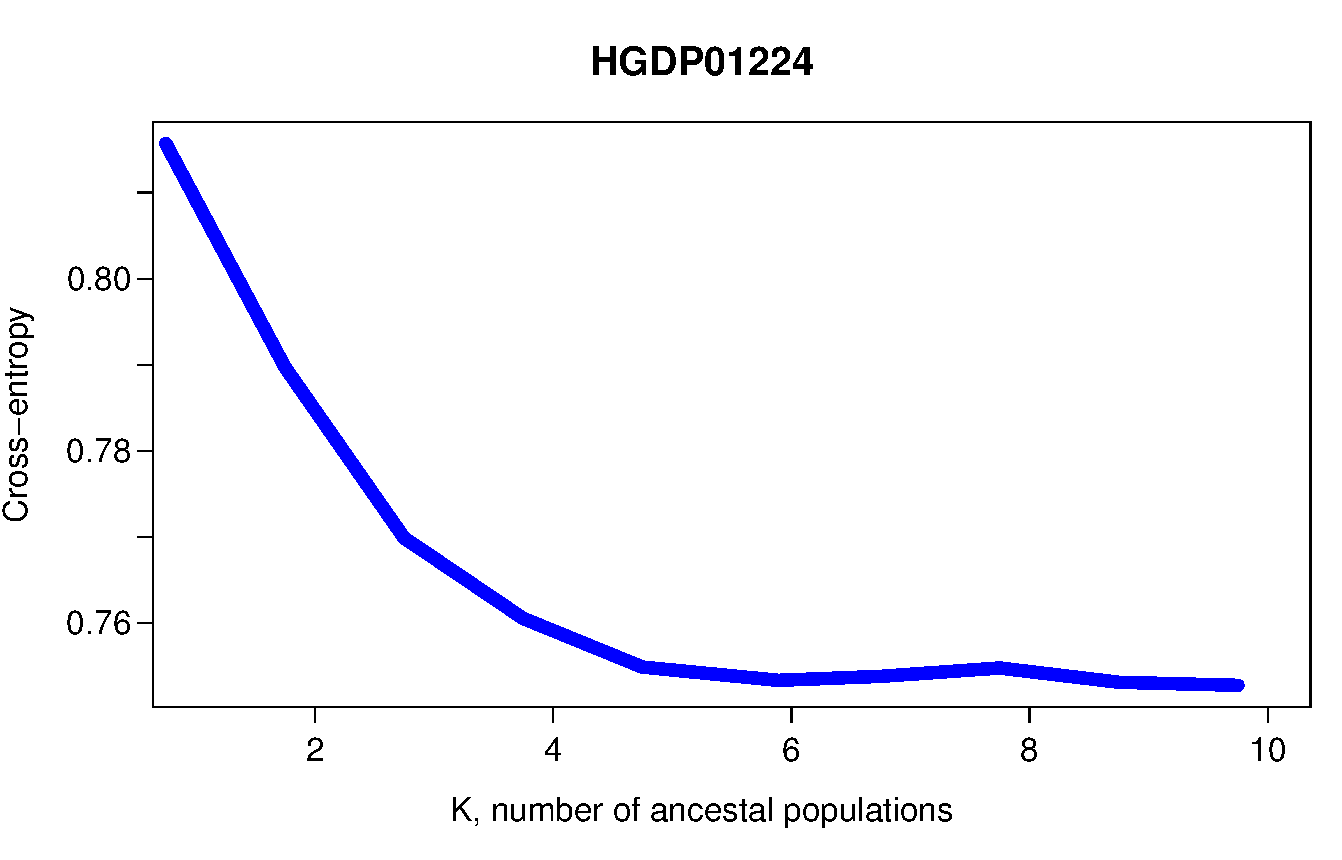
\includegraphics[width=15cm]{ce.pdf}}
\noindent{\bf Figure.}  {\bf Values of the cross-entropy criterion for 10 {\tt sNMF} runs (dataset HGDP01224).} 
\\
\\

\noindent
The ancestry coefficients for $K=6$ are available in the file examples/panel11.6.Q. The format of the file containing the ancestry coefficients is the format used by the software {\tt STRUCTURE}. This file can be used as input into CLUMPP, the software to gather output runs [3] and into distruct to display admixture plots [4].\\
\\
\noindent
Below, the first three lines of examples/panel11.6.Q.
\begin{center}
\footnotesize
\begin{Verbatim}[frame=single]
0.150569 0.0135955 0.0103463 0.779787 0.00755981 0.0381422
0.156673 0.0584628 0.0543375 0.682024 9.9991E-05 0.0484029
0.280393 0.00873713 0.0120376 0.635205 0.0635271 9.9991E-05
\end{Verbatim}
\end{center}
{\it Tips:} It is clearly useful to perform several runs of {\tt sNMF} for the same value of $K$ and to choose the run with the smallest value of the cross-entropy criterion.



\section{Contact}
If you need assistance, do not hesitate to send us an email (eric.frichot@imag.fr or olivier.francois@imag.fr). 
A FAQ (Frequently Asked Questions) section is available 
on our webpage (http://membres-timc.imag.fr/Olivier.Francois/snmf.html). 
{\tt sNMF} software is still under development. All your comments and feedbacks are more than welcome.\\
\\
\noindent
[1] Eric Frichot, François Mathieu, Théo Trouillon, Guillaume Bouchard, Olivier François. (2014) {\it Fast and efficient estimation of individual ancestry coefficients}. Genetics 196: 973 -- 983.\\ 
\\
\noindent
[2]  Nick J. Patterson, Priya Moorjani, Yontao Luo, Swapan Mallick, Nadin Rohland, Yiping Zhan, Teri
Genschoreck, Teresa Webster, and David Reich. (2012) {\it Ancient admixture in human history}. Genetics
192: 1065 -- 1093.\\
\\
\noindent
[3] Mattias Jakobsson, Noah A. Rosenberg. (2007) {\it CLUMPP: a cluster matching and permutation program for dealing with label switching and multimodality in analysis of population structure}. Bioinformatics, 23(14): 1801--1806.
\\
\\
\noindent
[4] Noah A. Rosenberg. (2004) {\it DISTRUCT: a program for the graphical display of population structure}. Molecular Ecology Notes, 4(1): 137--138.

\end{document}
